\chapter{Analisi dati}
\section{Statistiche generali}
I dati analizzati comprendono le transazioni dal \textbf{3 Gennaio 2009} al \textbf{10 Agosto 2017}.

Come spiegato precedentemente il primo obiettivo è quello di presentare statistiche generali sull'uso del dust, mostrare gli effetti del dust sulla de-anonimizzazione di address e infine descrivere due pattern che potrebbero rappresentare dei Dust Attack.

Per questo motivo il primo compito è stato il filtraggio di tutte le transazioni dust, ovvero tutte quelle transazioni che comprendono tra gli input e/o tra gli output un importo $<$ 546 satoshi.
\begin{figure}[H]
\begin{mdframed}
 infos:inputs:118890,\textbf{99},2;118902,9987098901,2 \checkmark\\
 infos:21482214,984902,114569039,1;21482868,\textbf{1},73028796,240:outputs \checkmark\\
 infos:118925,9963398109,121409,0:118926,9962398010,2 \textbf{x}
\end{mdframed}
\caption{Esempi di transazioni accettate o rifiutate}
\label{tx_dust}
\end{figure}
\Floatbarrier
La figura \ref{tx_dust} mostra due esempi di transazioni dust e un esempio di transazione non-dust, le prime due transazioni vengono considerate nelle analisi successive proprio perchè contengono importi dust. 

La prima infatti contiene, tra gli output, un importo di 99 satoshi, la seconda invece contiene un importo di 1 satoshi tra gli input. L'ultima transazione invece è stata scartata proprio perchè tutti gli importi sono $\ge$ 546 satoshi. Le transazioni non-dust di qusto tipo sono state ignorate poichè le analisi vertono sulla generazione e sul consumo del dust e sulla de-anonimizzazione causata da questi importi.

Le transazioni totali sono 245 410 083 mentre le transazioni che generano o consumano dust sono  2 114 335, questo significa che il dust è presente solo nello 0.8\% delle transazioni totali; inoltre come riportato in \cite{dustAnalisi} 1 705 560 creano dust mentre solo 429 544 lo consumano. Da questi due ultimi risultati possiamo dedurre che ci sono transazioni in cui il dust è presente sia negli input che negli output.

Il passaggio successivo è stato il filtraggio delle transazioni generate da Satoshi Dice. Satoshi Dice, come spiegato in precedenza, è un noto servizio di gambling nato nell'Aprile 2012; questo servizio utilizza il dust per comunicare ai giocatori perdenti che hanno perso la loro scommessa. Data la notorietà del servizio risulta molto poco probabile che l'intento sia quello di un Dust Attack, inoltre le analisi vogliono mostrare il comportamento degli utenti nei confonti del dust proveniente da address sconosciuti; gli address di Satoshi Dice sono noti proprio perchè il servizio stesso li ha resi pubblici.

Le transazioni generate da Satoshi Dice sono 1 465 295, ovvero il 69\% delle transazioni dust. Questo risultato, oltre a dimostrare la popolarità del servizio, permette di concentrare le future analisi sul rimanente 31\%(649 040) delle transazioni.

Una volta ottenute tutte e sole le transazioni di interesse sono stati realizzati gli istogrammi mostrati in figura \ref{fig:dust_distribuzione}. Il primo istogramma mostra la distribuzione del numero di input dust, il secondo invece la distribuzione del numero di output. In entrambi i grafici non sono state contate le transazioni con 0 importi dust. La prima colonna infatti rappresenta, in entrambi gli istogrammi, l'intervallo [1, 50].
\begin{figure}[h!]
    \centering
    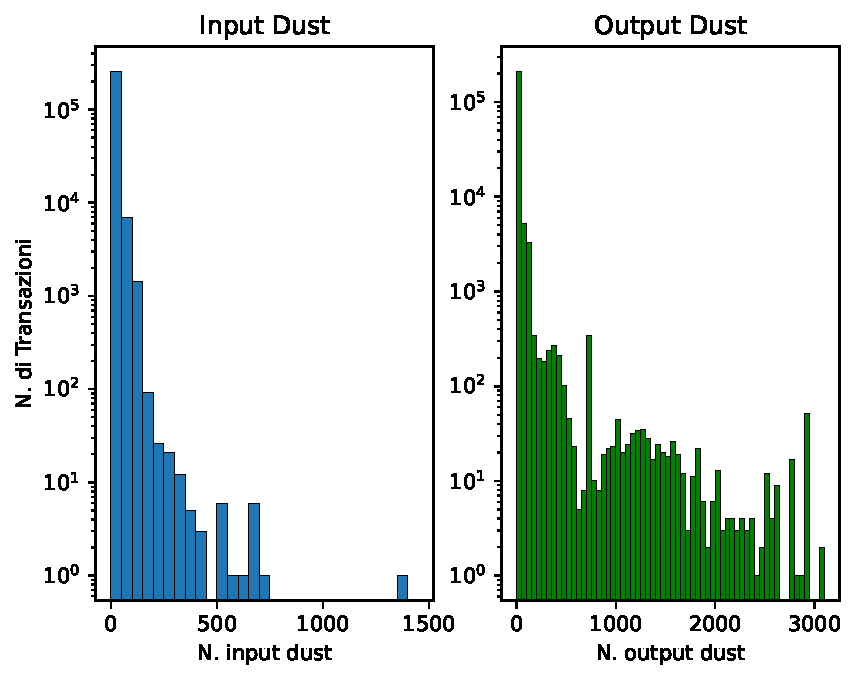
\includegraphics[scale=0.9]{Grafici/distribuzione_dust.pdf}
    \caption{Distribuzione numero input dust(sinistra) e output dust(destra)}
    \label{fig:dust_distribuzione}
    \subcaption{Intervalli di ampiezza 50}
    \subcaption{Primo intervallo [1, 50]}
\end{figure}
\FloatBarrier 
Entrambi gli istogrammi mostrano come siano molto frequenti le transazioni presenti nel primo intervallo di ampiezza [1, 50]. Nel primo grafico però notiamo anche che le transazioni con un elevato numero di input dust risultino poco usuali. Al contrario del primo grafico il secondo mostra come siano presenti tante transazioni che generano un elevato numero di output dust. Da questi due grafici inoltre possiamo già intuire che diversi output dust generati non vengano successivamente spesi.

Nelle analisi successive viene ignorato il dust generato con script OP\_RETURN. Questa scelta è motivata dal fatto che gli output con questo script non possono essere spesi, questa tipologia di dust quindi non può avere effetti sulla de-anonimizzazione; inoltre chi lo sta generando sicuramente non sta attuando un Dust Attack.

Il grafico \ref{fig:dust_created} mostra la generazione nel tempo del dust spendibile.
\begin{figure}[h!]
    \centering
    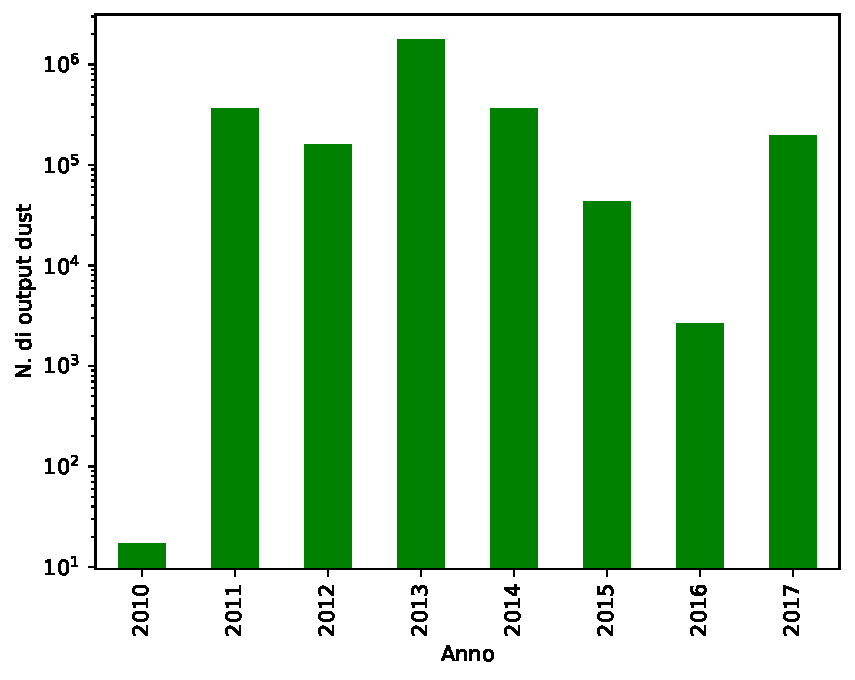
\includegraphics[scale=0.9]{Grafici/dust_created_year.pdf}
    \caption{Creazione dust nel tempo}
    \label{fig:dust_created}
\end{figure}
\FloatBarrier 
Dal grafico è possibile notare che già dal 2010 sono comparsi i primi output dust, anche se in quantità molto ridotta. Possiamo osservare una rapida salita tra il 2010 e il 2011, solo nel mese di luglio infatti sono stati generati 27 376 output dust.

Il picco della generazione di dust lo abbiamo nel 2013, dove sono state trovate transazioni legate "a catena"; nel paragrafo successivo verrà approfondito questo schema. Dopo il picco del 2013 osserviamo una diminuzione negli anni fino al 2017 dove sembrerebbe esserci una ricrescita. Bisogna però specificare che la maggior parte del dust generato nel 2017 proviene da due address: 1Enjoy1C4bYBr3tN4sMKxvvJDqG8NkdR4Z e 1SochiWwFFySPjQoi2biVftXn8NRPCSQC.

Questi due noti address sono comparsi per la prima volta nel 2014, in concomitanza con le olimpiadi di Sochi in Russia, generando transazioni con circa 750 output di 1 satoshi ciascuno. È importante notare che, nonostante il caos causato in vari forum Bitcoin, la tempesta di spam del 2014 "Enjoy Sochi" ha lasciato una piccola impronta sulla blockchain; solo 65 transazioni(48 750 output dust) sono state confermate in quell'anno.

L'aspetto singolare di questo fenomeno è che abbiamo visto echi di esso tornare negli anni successivi. Nel 2015 infatti sono state confermate 23 transazioni(1 725 output dust) mentre nel 2017 sono presenti 255 transazioni(191 250 output dust) generate da 1Sochi e 1Enjoy. Sebbene sia possibile che vengano eseguite dalla stessa entità, che spendeva importi da quegli address anche nel 2018, è anche possibile che queste transazioni fossero state generate nel 2014 e confermate solo nel 2015 e nel 2017. In questi tre anni il fenomeno "Enjoy Sochi" ha generato 343 transazioni per un totale di output dust intorno ai 255 000.

In generale sono stati generati 2 893 877 output dust con script diverso da OP\_RETURN; circa il 48.5\% è stato speso. Quindi non è presente una grande differenza tra la quantità di dust non speso(51.5\%) e la quantità di dust speso. 

La tabella \ref{tab:dust_spent_unspent} mostra le percentuali negli anni del dust speso e non-speso; il 2009 non è stato considerato perchè non è stato generato alcun output dust in quell'anno. La superiorità del dust non-speso rispetto al dust speso deriva quindi soprattutto dagli anni 2011 e 2017, anche se parte del dust del 2017 potrebbe essere stato speso successivamente al 10 Agosto 2017, data dell'ultima transazione del dataset. Il 2010, nonostante il dust non-speso sia l'83\%, non è molto rilevante poichè sono stati generati solo 14 output dust in totale. 
\begin{table}[H]
    \centering
    \begin{tabular}{|c|c|c|c|c|c|c|c|c|}
        \hline
           categoria/anno   & 2010 & 2011 & 2012 & 2013 & 2014 & 2015 & 2016 & 2017\\
        \hline 
         speso &  17\% & 0,2\% & 54\% & 44\% & 76\% & 94,6\% & 95,6\% & 10\% \\
         \hline
         non-speso & 83\% & 99,8\% & 46\% & 56\% & 24\% & 5,4\% & 4,4\% & 90\%  \\
         \hline
    \end{tabular}
    \caption{Dust Speso e Non-Speso negli anni}
    \label{tab:dust_spent_unspent}
\end{table}
Gli output dust sono stati suddivisi in quattro categorie:
\begin{enumerate}
    \item \textbf{Successo}: dust speso in transazioni che presentano almeno due address di input la cui fee è diversa dall'importo totale di input;
    \item \textbf{Fallimento}: dust speso in transazioni con un solo address di input;
    \item \textbf{Speciale}: dust speso in possibili transazioni di ``dust collecting", transazioni la cui fee è uguale all'importo totale di input;
    \item \textbf{Non speso}.
\end{enumerate}
I termini "Successo" e "Fallimento" si riferiscono alla possibilità di collegare gli address di input una volta che il dust è stato speso. Nonostante il ``dust-collecting" rappresenti un caso di de-anonimizzazione fallita, gli address di input infatti potrebbero appartenere ad utenti diversi, viene separata dalla categoria ``Fallimento" per mostrare se e quanto sia stato utilizzato questo servizio.

Il grafico \ref{fig:dust_year} mostra quanto siano presenti le categorie nel corso degli anni.
\begin{figure}[h!]
    \centering
    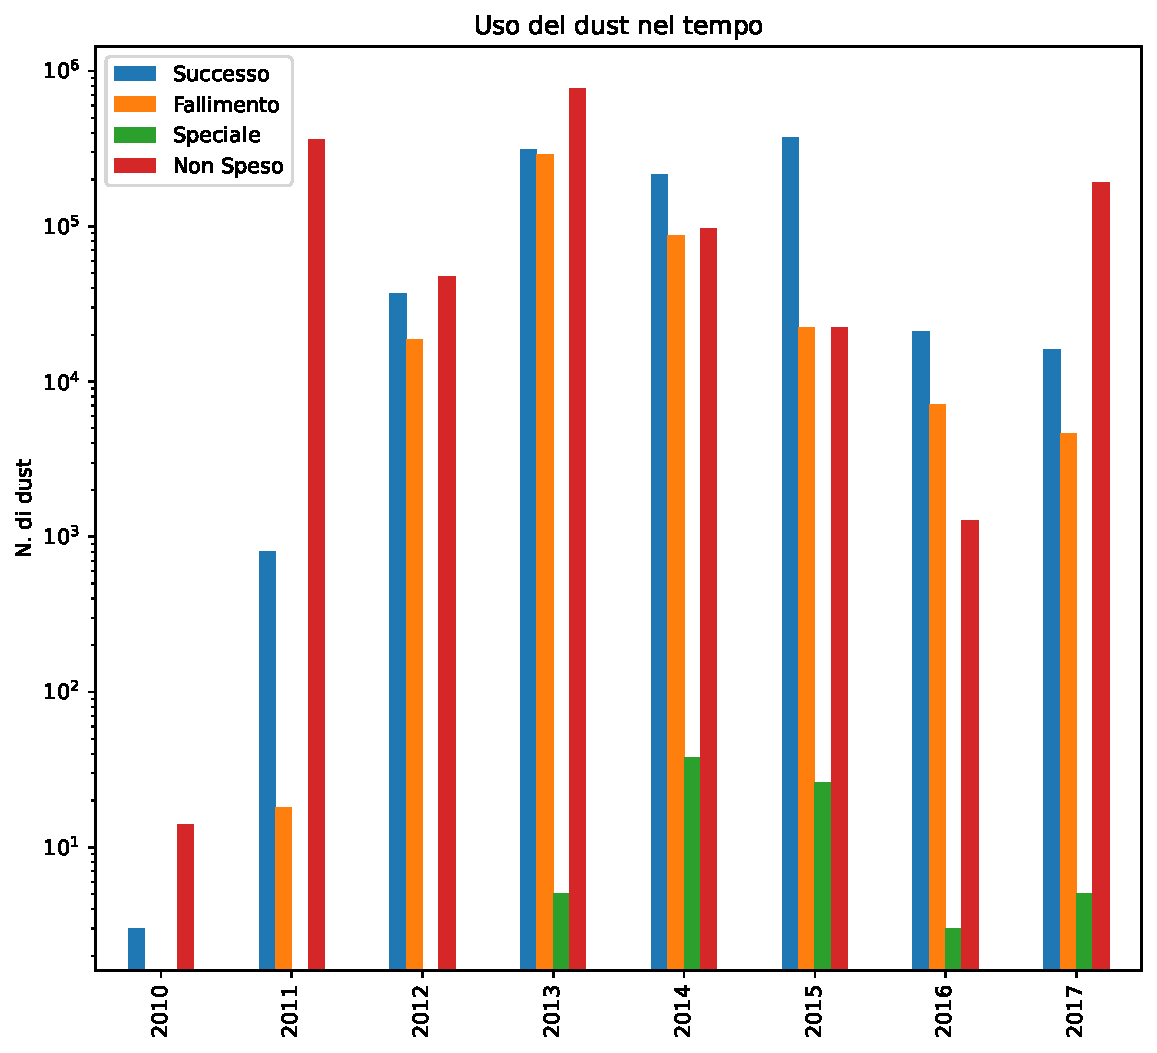
\includegraphics[scale=0.6]{Grafici/uso_del_dust_new.pdf}
    \caption{Uso del dust nel tempo}
    \label{fig:dust_year}
\end{figure}
\FloatBarrier
Non solo possiamo constatare graficamente quanto detto prima sulla differenza tra dust speso e non speso, ma possiamo anche trarre due importanti riflessioni. 

La prima riguarda l'uso del ``dust collecting", risulta evidente quanto poco sia stato utilizzato questo servizio. Il dust della categoria ``Speciale" non necessariamente è legato a Dust-B-Gone, questa categoria infatti è presente anche nel 2017 nonostante il servizio sia stato ufficialmente chiuso nel 2016. Se un utente decidesse di sua iniziativa di spendere tutto il dust in fee rientrerebbe comunque in questa categoria.

In generale infatti non è possibile distinguere una transazione di ``dust-collecting" da una transazione generata da un singolo utente, ma il numero di dust della categoria ''Speciale" costituisce un limite superiore al numero di dust spesi tramite Dust-B-Gone.

La seconda riflessione invece riguarda la tendenza a spendere il dust con almeno un altro address, in particolare notiamo un netto distacco nel 2015 dove la categoria ”Successo” rientra nell’ordine di $10^4$ mentre ”Fallimento” nell’ordine di $10^3$. In generale questa informazione è molto importante perchè dimostra come il dust possa essere efficace per la de-anonimizzazione di un wallet, ovvero capire che più address appartengano ad un medesimo utente.

Una volta constatata la presenza di transazioni con input dust e con almeno due address diversi, la fase seguente è l'analisi delle transazioni. 

Abbiamo tre categorie di transazioni: 
\begin{itemize}
    \item \textbf{2+ address}: transazioni che presentano almeno due address di input differenti, la fee però è diversa dall'importo totale di input;
    \item \textbf{1 address}: transazioni con un singolo address di input;
    \item \textbf{speciale}: transazioni dove l'importo totale di input è uguale alla fee.
\end{itemize}

In totale il dust è stato speso in 263 963 transazioni, la tabella \ref{tab:tx_categories} mostra la percentuale delle transazioni nelle tre categorie, la tabella \ref{tab:tx_categories_year} mostra una visione annuale.
\begin{table}[H]
    \centering
    \begin{tabular}{|c|c|}
        \hline
        2+ address & 63,2\%\\
        \hline
        1 address & 36,7\%\\
        \hline
        speciale & 0.1\%\\
        \hline
    \end{tabular}
    \caption{Transazioni nelle tre categorie}
    \label{tab:tx_categories}
\end{table}
\begin{table}[H]
    \centering
    \begin{tabular}{|l|c|c|c|c|c|c|c|c|}
        \hline
            categoria/anno  & 2010 & 2011 & 2012 & 2013 & 2014 & 2015 & 2016 & 2017\\
        \hline 
         2+ address(\%) & 100 & 93 & 55,6 & 68,4 & 55,9 & 64,5 & 62,7 & 75 \\
         \hline
         1 address(\%) & 0 & 7 & 44,4 & 31,5 & 44,09 & 35,4 & 37,2 & 24,7  \\
         \hline
         speciali(\%) & 0 & 0 & 0 & 0,1 & 0,01 & 0,1 & 0,1 & 0,3 \\
         \hline
    \end{tabular}
    \caption{Transazioni nel tempo}
    \label{tab:tx_categories_year}
\end{table}
Dalle tabelle \ref{tab:tx_categories} \ref{tab:tx_categories_year} confermiamo quanto detto prima, la prevalenza a spendere il dust in transazioni con almeno due address diversi e lo scarso utilizzo di servizi come Dust-B-Gone; la seconda fase delle analisi si concentrerà sui primi due gruppi.\\
La categoria "1 address" è stata ulteriormente suddivisa in due classi:
\begin{itemize}
    \item \textbf{NOD}: transazioni che presentanto input con importo $>$ 545  
    \item \textbf{OD}: transazioni con soli input dust.
\end{itemize}
Dalla tabella \ref{tab:OD_NOD_failed} possiamo dedurre che il fallimento nella de-anonimizzazione sia dovuto principalmente a quegli address che non sono vuoti, ovvero hanno ricevuto importi non-dust da altre fonti. 
\begin{table}[H]
    \centering
    \begin{tabular}{|c|c|c|}
        \hline
            NOD  & 92 712 & 95,5\%\\
        \hline 
            OD  & 4328 & 4,5 \%\\
        \hline
    \end{tabular}
    \caption{Classificazione OD e NOD}
    \label{tab:OD_NOD_failed}
\end{table}
Interessante invece è il secondo gruppo, in particolare due address: 1JwSSubhmg6iPtRjtyqhUYYH7bZg3Lfy1T e 1PEDJAibfNetJzM289oXsW1qLAgjYDjLgN. Il fatto interessante del primo address è che che la sua chiave privata è stata compromessa \footnote{fonte:\url{https://privatekeys.pw/address/bitcoin/1JwSSubhmg6iPtRjtyqhUYYH7bZg3Lfy1T}}, questo consente a chiunque di riscattare bitcoin non appena gli vengono inviati.\\\\
Caso anomalo invece riguarda 1PEDJAibfNetJzM289oXsW1qLAgjYDjLgN, rinominato 1PED per semplicità. Questo address, come riportato in \cite{dustAnalisi} è un noto gambler di Satoshi Dice, la singolarità però deriva da alcune transazioni che ha generato. In queste transazioni infatti è presente un solo input di 1 satoshi e un solo output, ovviamente sempre di 1 satoshi. Questi singoli satoshi però non provengono da Satoshi Dice ma da altri address che seguono un pattern ben preciso, schematizzato nella figura \ref{fig:1PED}
\begin{figure}[h!]
    \centering
    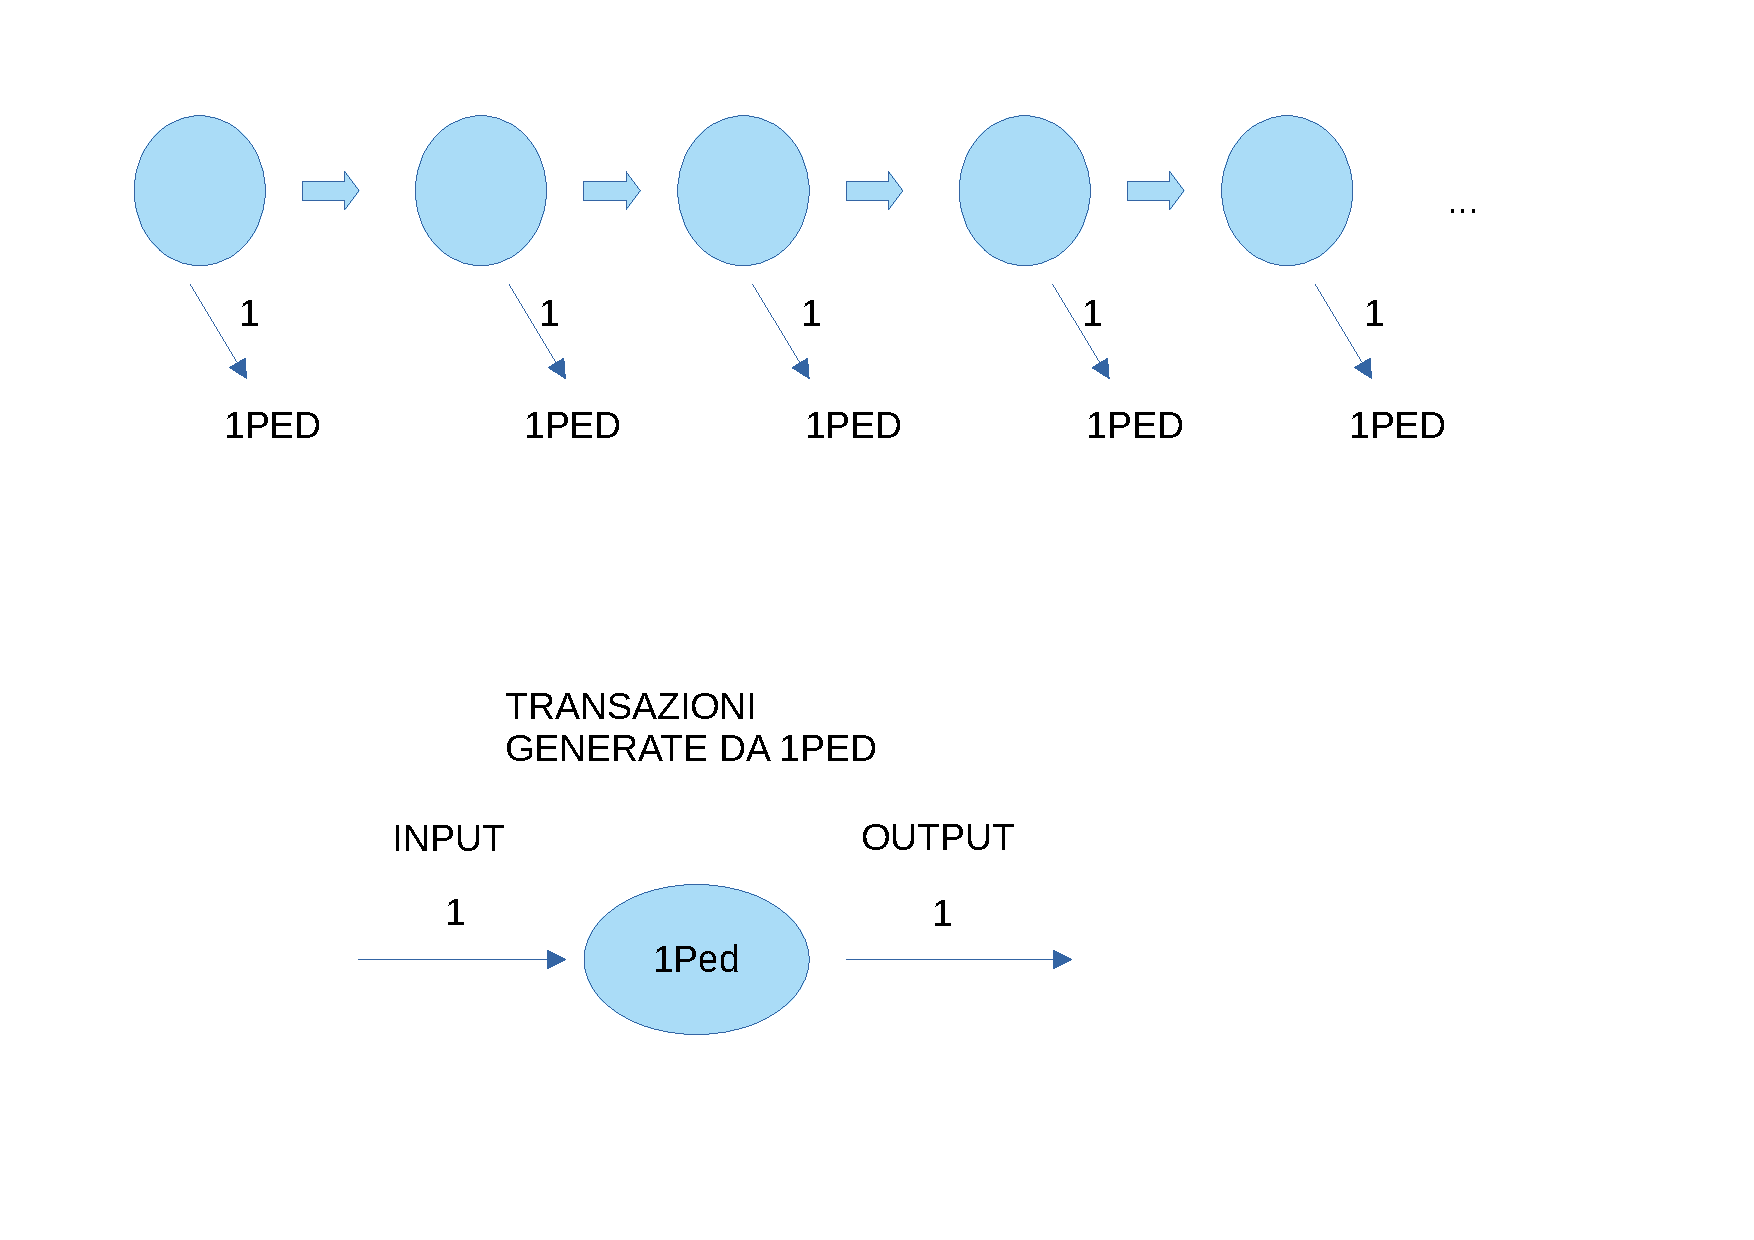
\includegraphics[scale=0.4]{Images/1Ped.pdf}
    \caption{Schema transazioni legate a 1PED}
    \label{fig:1PED}
\end{figure}
\FloatBarrier
Ogni address invia due output, 1 satoshi con destinatario 1PED e un secondo importo che viene inviato ad un altro address che seguirà il medesimo schema; in tutte queste transazioni la fee è di 50 000 satoshi. 1PED ha generato poi 1835 transazioni con 1 solo satoshi di input e 1 solo satoshi di output, la data è il 10 Marzo 2013 alle ore 16:20. Gli address destinatari però compaiono nella blockchain per la prima volta proprio grazie a queste transazioni, sicuramente non si tratta di un tentativo di Dust Attack.\\\\
Molto più interessanti sono le transazioni della categoria "2+ address". Anche in questo caso vengono mostrati i gruppi OD e NOD. La tabella \ref{tab:OD_NOD_success} mostra come quasi sempre si riescano a collegare address vittima di dust con address più capienti.
\begin{table}[H]
    \centering
    \begin{tabular}{|c|c|c|}
        \hline
            NOD  & 166 778 & 99,9\%\\
        \hline 
            OD  & 128 & 0,1 \%\\
        \hline
    \end{tabular}
    \caption{Classificazione OD e NOD}
    \label{tab:OD_NOD_success}
\end{table}
È importante però capire quanto successo abbia avuto la de-anonimizzazione, la tabella \ref{tab:stat} mostra alcune statistiche generali di questa categoria. 
\begin{table}[H]
    \centering
    \begin{tabular}{|c|c|}
        \hline
            Percentuale media numero input dust & 29 \%\\
        \hline
            Moda percentuale numero input dust & 50 \%\\ %18 187 tx così
        \hline
            Media numero address diversi & 13\\
        \hline
            Moda numero address diversi & 2\\ %35011
        \hline
    \end{tabular}
    \caption{Statistiche generali}
    \label{tab:stat}
\end{table}
Possiamo subito osservare come moda e media tendano ad essere molto diverse tra loro, questo fatto permette di capire come le transazioni più frequenti non siano dominanti. In entrambe le situazioni infatti le transazioni che costituiscono la moda corrispondono a circa il 10\% nel primo caso(percentuale media numero di input dust) e al 20\% nell'ultimo(numero di address diversi). I grafici \ref{fig:distribuzioni_tx} mostrano, partendo da sinistra, la distribuzione della percentuale di input dust e la distribuzione degli address diversi. Nel primo istogramma le colonne rappresentano gruppi di 0,10, nel secondo invece gruppi di 50.
 \begin{figure}[h!]
     \centering
     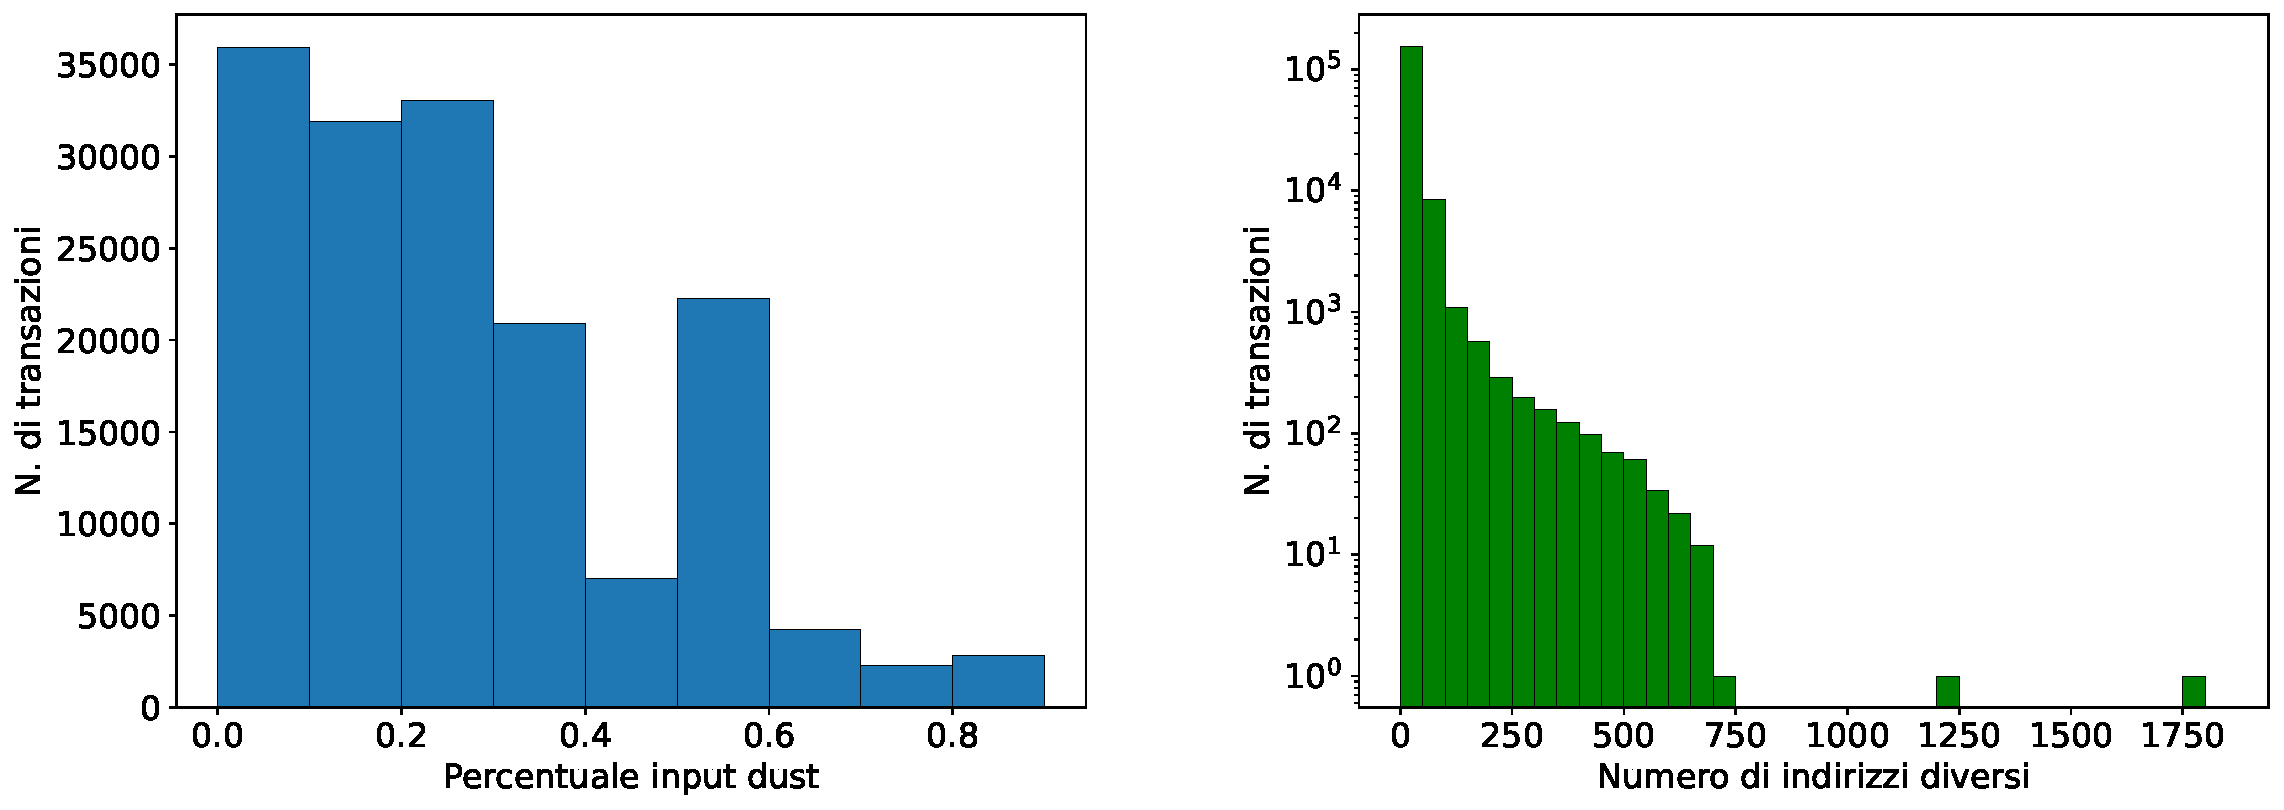
\includegraphics[scale=0.44]{Grafici/Distribuzioni_belle.pdf}
     \caption{Distribuzione percentuale input dust(sinistra), distribuzione address diversi(destra)}
    \label{fig:distribuzioni_tx}
 \end{figure}
\FloatBarrier
Dal primo istogramma notiamo la prevalenza degli input non-dust rispetto a quelli dust, la maggior parte della transazioni infatti ha una percentuale di input dust inferiore al 40\%. Questo dato è molto importante perchè mostra come il dust permetta di collegare soprattutto address più capienti, che potrebbero essere di maggiore interesse per un possibile attaccante. Il secondo istogramma invece mostra come siano presenti molte transazioni con un elevato numero di address diversi, permettendo un'efficace de-anonimizzazione dei relativi wallet.\\\\
È importante precisare che stessi address possano apparire in più transazioni, potrebbero quindi esserci delle de-anonimizzazioni ripetute. Infatti nonostante siano stati generati 2 893 877 output dust gli address a cui sono stati inviati sono 1 059 836 e solo il 29\%(312 114) lo ha speso. Di questo 29\% abbiamo che 259 252 hanno speso il dust in transazioni della categoria "2+ address" anche se 4 270 address hanno anche generato transazioni nella categoria "1 address". Una particolarità interessante delle transazioni che hanno generato il dust "Successo" è che in molti casi erano presenti tra gli output dust address nuovi, ovvero address che non erano mai comparsi sulla blockchain. Ci sono 98 198 transazioni che generano almeno un dust della categoria "Successo", circa il 59\%(58 146) non presenta address nuovi tra gli output. Nella fase finale delle analisi sono state prese queste transazioni così da trovare dei pattern interessanti di possibili Dust Attack di successo; nel paragrafo successivo verranno approfonditi due possibili schemi di Dust Attack.  
\section{Pattern Interessanti}
In generale è complicato affermare con certezza se un address stia compiendo un Dust Attack, però sono presenti due schemi, con certe proprietà, che potrebbero rappresentare un Dust Attack. La proprietà più importante riguarda l'assenza di address nuovi tra gli output dust, proprio perchè è alquanto improbabile tentare di de-anonimizzare un address mai visto fino a quel punto.\\
Il primo pattern, sintetizzato in \ref{fig:schema1}, risulta molto simile al caso 1PED. Abbiamo diversi address legati a catena che generano transazioni bi-output. Il secondo output, inviato al solito address, viene speso dall'attaccante per generare transazioni contenenti solo output dust. Inoltre l'attaccante, nell'immagine l'ovale rosso, non compare mai nella catena dei finanziatori, rappresentata dai cerchi azzurri.
\begin{figure}[h!]
    \centering
    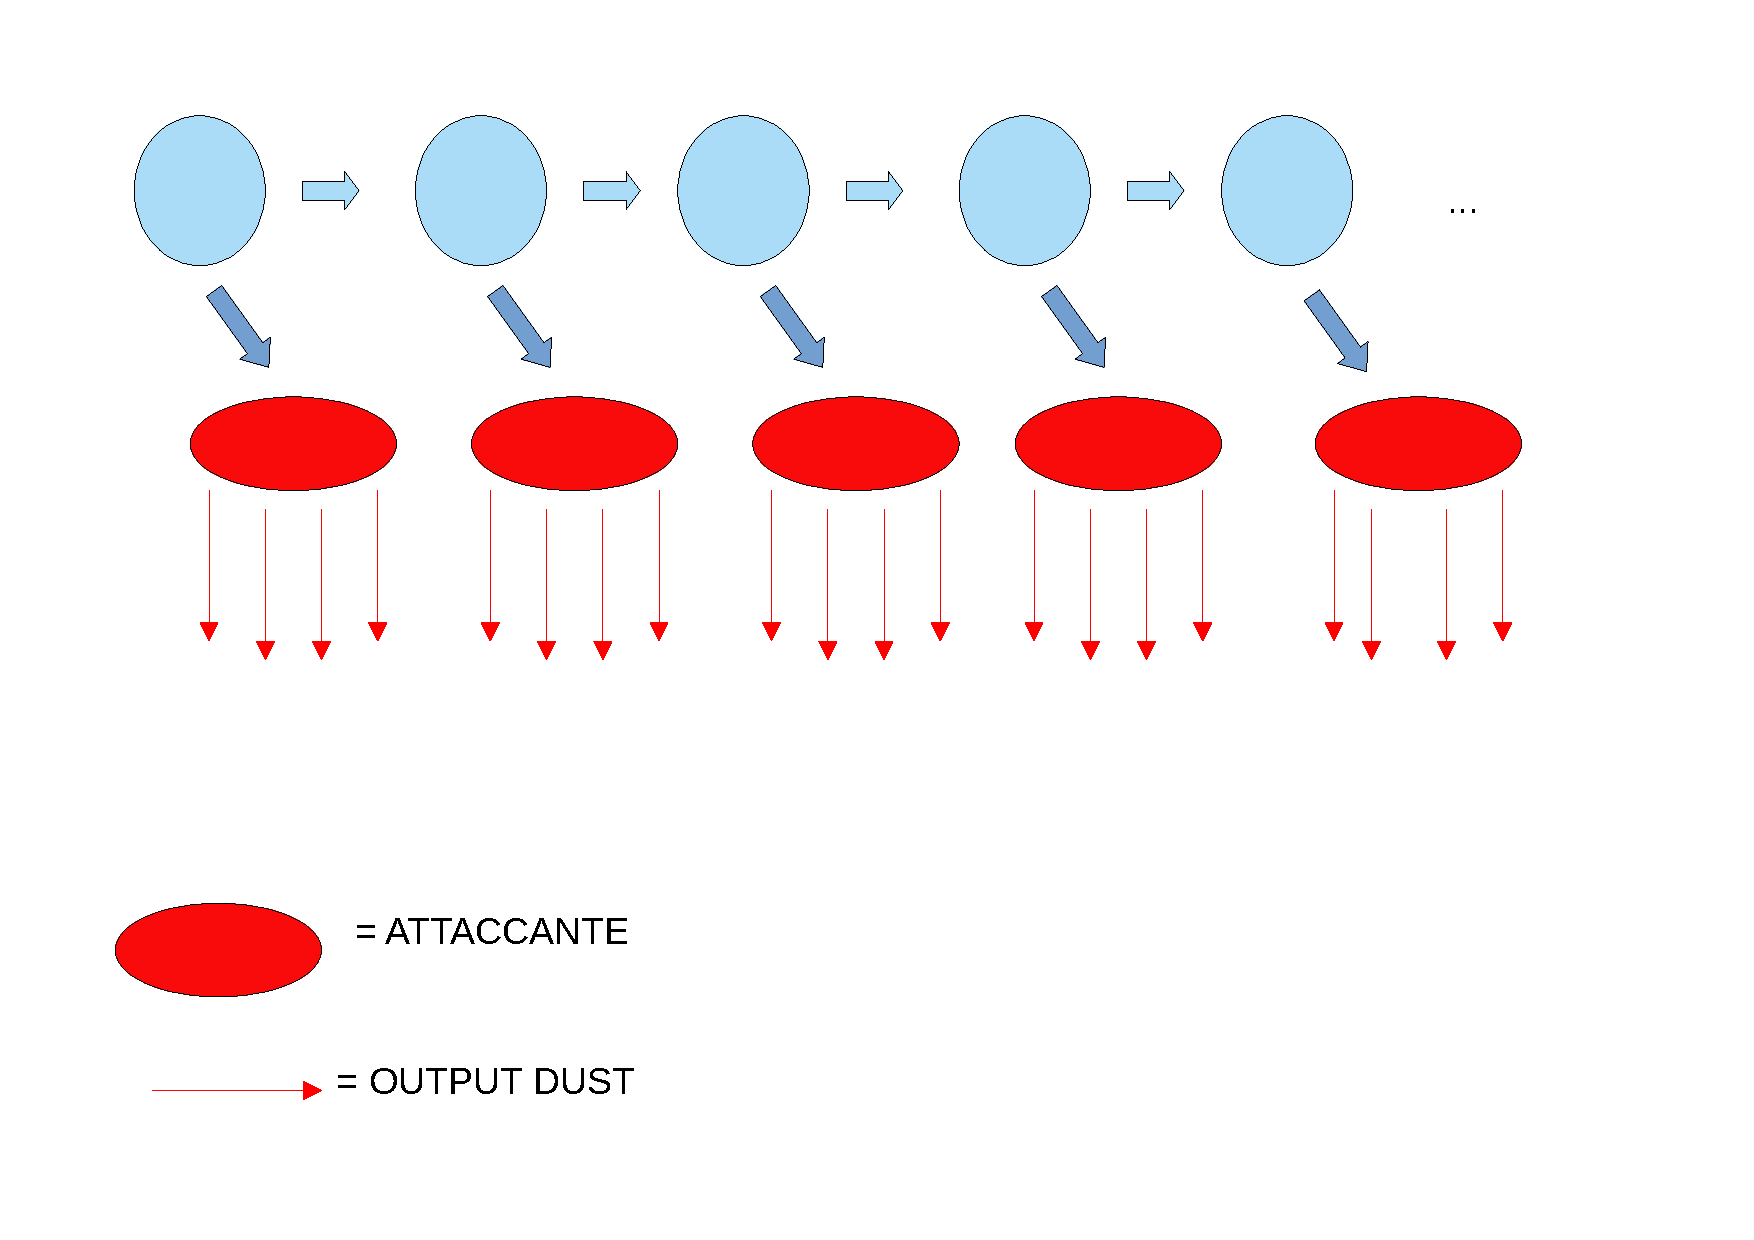
\includegraphics[scale=0.4]{Images/dust_attack1.pdf}
    \caption{Primo Pattern}
    \label{fig:schema1}
\end{figure}
\FloatBarrier
Altre proprietà importanti di questo pattern sono: avere un unico finanziatore, generare sempre lo stesso numero di output dust, avere sempre il medesimo importo di input e infine l'attaccante esegue le transazioni in un breve intervallo di tempo. Questo schema è stato scoperto tramite l'address 1DiRy9Giiq1GCkAD7VMSrXoKVe2dimnovm, finanziato da 1Nj3AsYfhHC4zVv1HHH4FzsYWeZSeVC8vj. Inoltre sono presenti altri address che seguono lo stesso schema, pagati sempre dallo stesso finanziatore di 1Diry. Questo significa che il pattern appena enunciato può essere eseguito in parallelo utilizzano diversi address attaccanti. Potrebbero esserci in aggiunta più finanziatori che inviano denaro a più attaccanti. Per esempio questo address 16JLbXYe5xmxGNX8hiqooyTUJnhitNNqTh ha ricevuto fondi da 1NPfnbqZAMUnGuNuYwVZdCN4qVzUq4ejG4, l'aspetto interessante però è che il numero di output dust, l'importo dust inviato, l'importo input speso sono esattamente uguali a quelli usati da 1Diry; questo fatto fa ipotizzare che probabilmente questi address appartengano alla stessa persona. Ovviamente possono esserci eccezioni a questi due esempi trovati, per esempio avere più finanziatori o più attaccanti in una stessa catena, inoltre gli importi e il numero di output dust potrebbero avere una natura più randomica. In generale si potrebbero ipotizzare diverse variazioni di questo pattern, ovviamente ciò non implica che siano presenti.\\\\
Il secondo pattern, scoperto tramite 1JYvvL67LrSGCG77cy4rmpUXCFfSub4JkG (rinominato 1Jyvv), riguarda le transazioni "a catena" del 2013 citate nel paragrafo precedente. Ogni address della catena invia centinaia o migliaia di output dust e parte dell'importo, la fee è sempre $>$ 0, viene inviato al prossimo address che seguirà lo stesso schema. La singolarità di questo modello è che gli address della catena, ad eccezione del primo, vengono utilizzati solo per eseguire quell'unica transazione, non verranno mai più riutilizzati.
\begin{figure}[h!]
    \centering
    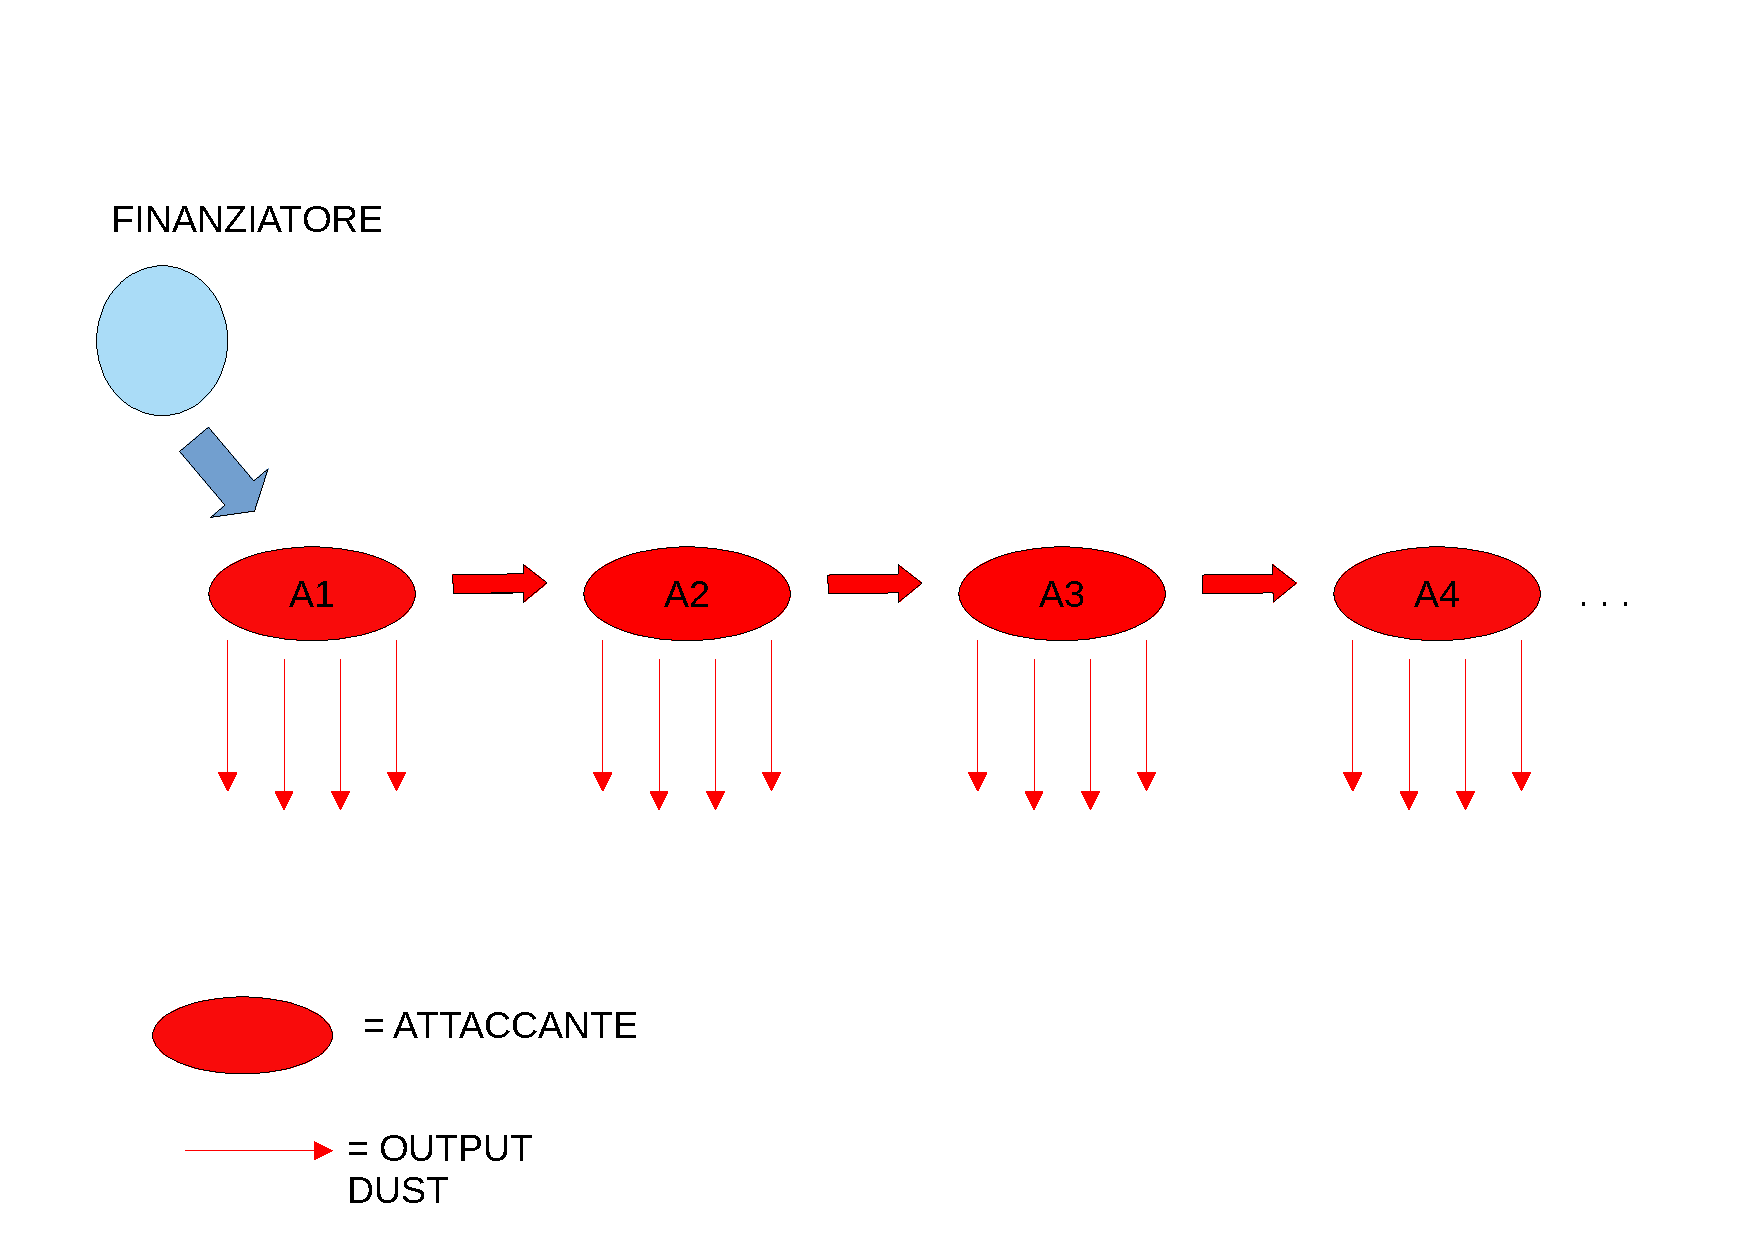
\includegraphics[scale=0.4]{Images/dust_attack2.pdf}
    \caption{Secondo Pattern}
    \label{fig:schema2}
\end{figure}
\FloatBarrier
Prendiamo come esempio l'address A3 della figura \ref{fig:schema2}. A3 compare in sole due transazioni. Nella prima, generata da A2, appare come destinatario di un importo non-dust, nella seconda invece spende questo importo inviando centinaia o migliaia di output dust e un importo non-dust con destinatario A4. Questo discorso però non si applica a colui che inizia questo pattern(A1), per esempio l'address 1Jyvv ha cominciato una serie di catene con questo modello.\\Potrebbe essere interessante in futuro capire quanti address abbiano seguito schemi di questi tipo e se ci siano altri fini oltre a quello di un possibile Dust Attack.